\hypertarget{adding-tests-to-legacy-code}{%
\section{Adding tests to legacy
code}\label{adding-tests-to-legacy-code}}

\begin{tcolorbox}[colback=blue!5!white,colframe=blue!75!black]
You

\begin{itemize}
\tightlist
\item
  know the difficulties of adding tests to existing code
\item
  know methods and techniques to add tests to existing code
\item
  know and can apply dependency-breaking techniques to add tests
\end{itemize}
\end{tcolorbox}

\hypertarget{test-driven-development}{%
\subsection{Test Driven Development}\label{test-driven-development}}

\begin{figure}[H]
\centering
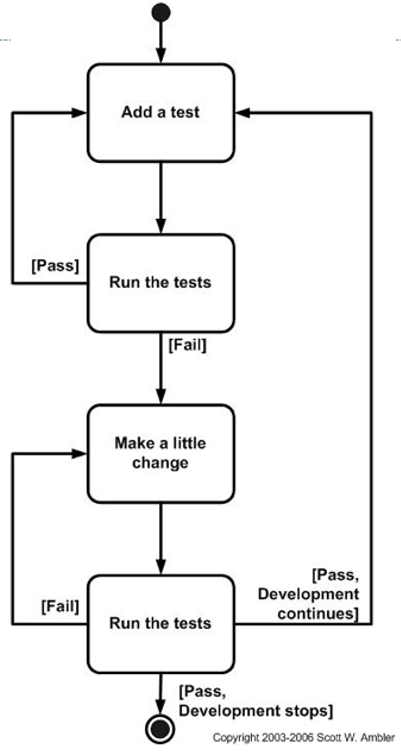
\includegraphics[width=0.3\textwidth]{figures/tdd.png}
\caption{Test Driven Development}
\end{figure}

\begin{itemize}
\tightlist
\item
  Test Driven Development is not only about testing!
\item
  Test Driven Development is also about design and documentation!
\item
  Writing the test cases for a class gives you the point of view of its
  clients.
\item
  Test Driven Development helps you design loosely coupled systems.
\end{itemize}

\begin{tcolorbox}[colback=red!5!white,colframe=red!75!black]
Writing tests is a design activity, it specifies each requirement in the form of an executable example that can be shown to work. These refactorings can be made with confidence because the test-first approach, by definition, guarantees a very high degree of test coverage to catch mistakes.
\end{tcolorbox}

\begin{tcolorbox}[colback=red!5!white,colframe=red!75!black]
Using TDD has many benefits but the most relevant is that it directs the programmer to think about the design of code from its intended use, rather than from its implementation.
\end{tcolorbox}

\hypertarget{isolation-in-tdd}{%
\subsubsection{Isolation in TDD}\label{isolation-in-tdd}}

It is important to isolate the class which should be tested.
Collaboration classes, databases or network resources should be replaces
by mock objects.

\begin{figure}[H]
\centering
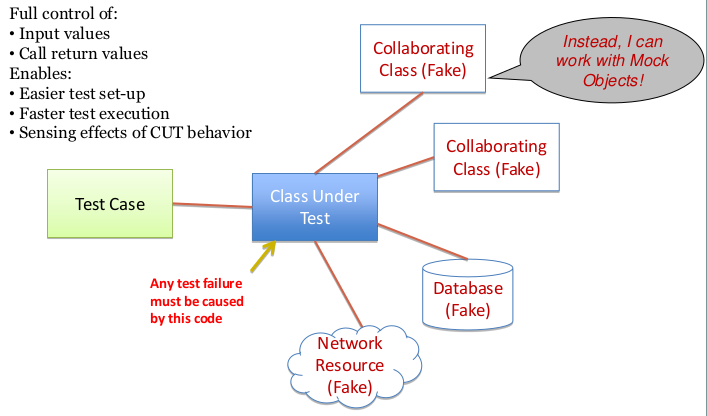
\includegraphics[width=0.5\textwidth]{figures/tdd_mocks.png}
\caption{Isolation in TDD}
\end{figure}

\hypertarget{repetition-what-is-legacy-code}{%
\subsubsection{Repetition: What is legacy
code}\label{repetition-what-is-legacy-code}}

\begin{itemize}
\tightlist
\item
  Code that has value\ldots{}
\item
  Code that we inherited\ldots{}
\item
  Code that is not fully documented, not necessarily perfectly
  designed\ldots{}
\item
  Untested Code
\item
  According to Feathers: "Legacy code is code that we've gotten from someone else. If you are at all like me, you think of tangled, unintelligible structure, code that you have to change but don't really understand."
\end{itemize}

\hypertarget{tdd-with-legacy-code}{%
\subsubsection{TDD with legacy code}\label{tdd-with-legacy-code}}

\begin{itemize}
\tightlist
\item
  Before changing a code snippet, I need a test for testing this snippet
\item
  Since I am not starting from scratch, it is possible that this snippet
  depends on other snippets
\item
  I need to break dependencies!
\end{itemize}

\begin{tcolorbox}[colback=red!5!white,colframe=red!75!black]
When we need to change code, we should have tests. To put tests in place, we often have to change code in advance.
\end{tcolorbox}

\hypertarget{legacy-change-algorithm}{%
\subsubsection{Legacy Change Algorithm}\label{legacy-change-algorithm}}

\begin{enumerate}
\def\labelenumi{\arabic{enumi}.}
\tightlist
\item
  Identify change points
\item
  Find test points
\item
  Break dependencies
\item
  Write tests
\item
  Make changes and refactor
\end{enumerate}

\hypertarget{sensing-and-seperation}{%
\subsubsection{Sensing and Seperation}\label{sensing-and-seperation}}

\textbf{Sensing:} we break dependencies to get some visibility into what
the code is actually doing. \\
\textbf{Separation:} we break dependencies
to be able to test a piece of code in isolation (without taking all
collaborating classes into the test harness)

\hypertarget{type-of-dependencies}{%
\paragraph{Type of Dependencies}\label{type-of-dependencies}}

\begin{itemize}
\tightlist
\item
  Singletons
\item
  Internal instanciations
\item
  Concrete Dependencies
\end{itemize}

\hypertarget{the-seam-model}{%
\subsubsection{The Seam Model}\label{the-seam-model}}

A seam is a place where you can alter behavior in your program without
editing in that place. Every seam has an enabling point, a place where
you can make the decision to use one behavior or another. That happens when you have an interface as a parameter. We do not know which object is behind that interface but everyone who implements it does have those functions. We do not know how it is implemented but it is.


\begin{figure}[H]
\centering
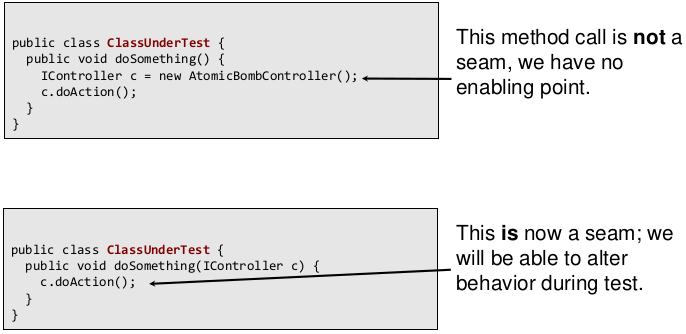
\includegraphics[width=0.5\textwidth]{figures/seamExample.png}
\caption{Seam Exampple}
\end{figure}


\clearpage
\hypertarget{dependency-breaking-techniques}{%
\subsection{Dependency Breaking
Techniques}\label{dependency-breaking-techniques}}

\hypertarget{extract-and-override-factory-method}{%
\subsubsection{Extract and Override Factory
Method}\label{extract-and-override-factory-method}}

\begin{itemize}
\tightlist
\item
  Identify the dependencies in the class which should be tested.
\item
  Extract all of the work involved in the dependency creation into a
  seperate factory method.
\item
  Create a testing subclass (of the class which should be tested) and
  override the factory method in it to inject your own dependency for
  the test.
\end{itemize}

\hypertarget{replace-global-reference-with-getter}{%
\subsubsection{Replace Global Reference with
Getter}\label{replace-global-reference-with-getter}}

\begin{itemize}
\tightlist
\item
  Identify the global reference that you want to replace.
\item
  Write a getter for the global reference. Make sure that the access
  protection of the getter is loose enough for you to be able to
  override the getter in a subclass.
\item
  Replace references to the global with calls to the getter.
\item
  Create a testing subclass and override the getter.
\end{itemize}

\hypertarget{extract-interface}{%
\subsubsection{Extract Interface}\label{extract-interface}}

\begin{enumerate}
\def\labelenumi{\arabic{enumi}.}
\tightlist
\item
  Find the member-functions that your class uses from the target class
\item
  Think of an interface name for the responsibility of those methods
\item
  Verify that no subclass of target class defines those functions
  non-virtually
\item
  Create an empty interface class with that name
\item
  Make the target class inherit from the interface class
\item
  Replace all target class references in the client class with the name
  of the interface
\item
  Lean on the Compiler to find the methods the interface needs
\item
  Copy function signatures for all unfound functions to the new
  interface. Make them pure virtual
\end{enumerate}

\hypertarget{parameterize-method}{%
\subsubsection{Parameterize Method}\label{parameterize-method}}

If a method has a hidden dependency on a class because it instantiates
it, make a new method that accepts an object of that class as an
argument.

\hypertarget{extract-and-override-call}{%
\subsubsection{Extract and Override
Call}\label{extract-and-override-call}}

When we have a bad dependency in a method and it is represented as a
call. We can extract the call to a method and then override it in a
testing subclass.

\begin{enumerate}
\def\labelenumi{\arabic{enumi}.}
\tightlist
\item
  Extract a method for the call (remember to preserve signatures)
\item
  Make the method virtual
\item
  Create a testing subclass that overrides that method
\end{enumerate}




\subsection{Inflection Point (Wendepunkt)}
After you found the place of the code you want to change, you need to find an Inflection Point. An Inflection Point is a narrow interface to a set of classes. If somebody change a class behind an inflection point, it will be detected at the inflection point.